\documentclass{beamer}
\usepackage{ArmenianSlides}

\begin{document}

\title[Mediator]{Նախագծման Ձևանմուշներ։ Mediator}
\author[Հրաչյա Թանդիլյան\copyright]{Հրաչյա Թանդիլյան}
\date{2020}

%-------------------------------------------------------------------------------------------------
\begin{frame}
\titlepage
\end{frame}
%-------------------------------------------------------------------------------------------------

\section{Նպատակը}
%-------------------------------------------------------------------------------------------------
\begin{frame}\frametitle{Mediator}
\begin{block}{Նպատակը}
    Սահմանել օբյեկտ, որը կինկապսուլացնի այն,\\
    թե ինչպես են փոխհամագործակցում մի խումբ օբյեկտներ: \\
    Այս Ն.Ձ. նպաստում է փոխկապակցվածության թուլացմանը, կանխելով օբյեկտների
    միմյանց ուղղակի հղվելու անհրաժեշտությունը և թույլ է տալիս անկախ կերպով փոփոխել
    նրանցով փոխազդեցությունը:
\end{block}
\vfill
Նաև հայտնի է որպես
\begin{itemize}
    \item Այլ լայնորեն կիրառվող անուներ չկան:
\end{itemize}
\end{frame}
%-------------------------------------------------------------------------------------------------

\subsection{Մոտիվացիան}
%-------------------------------------------------------------------------------------------------
\begin{frame}\frametitle{Մոտիվացիան}
\begin{center}
    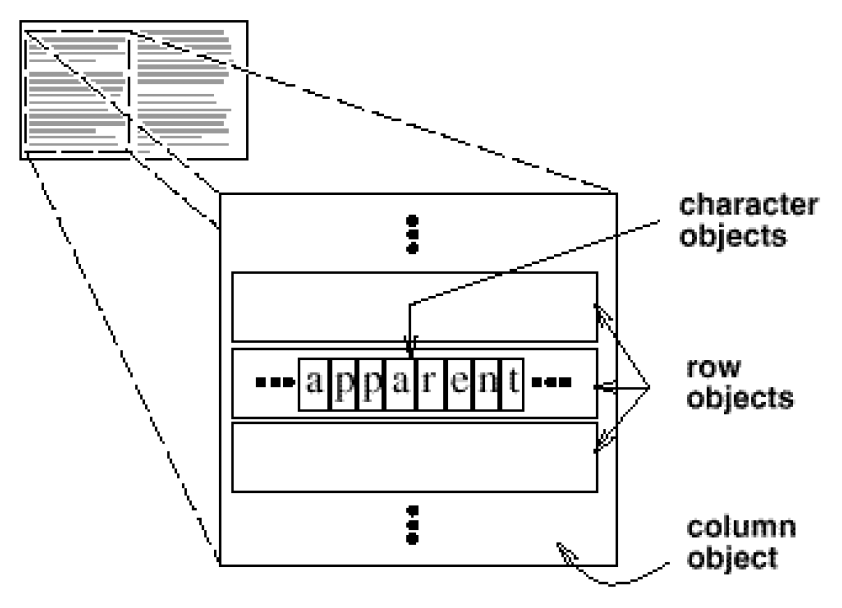
\includegraphics[scale=0.4]{motivation1.png}
\end{center}
\end{frame}
%-------------------------------------------------------------------------------------------------

%-------------------------------------------------------------------------------------------------
\begin{frame}\frametitle{Մոտիվացիան}
\begin{center}
    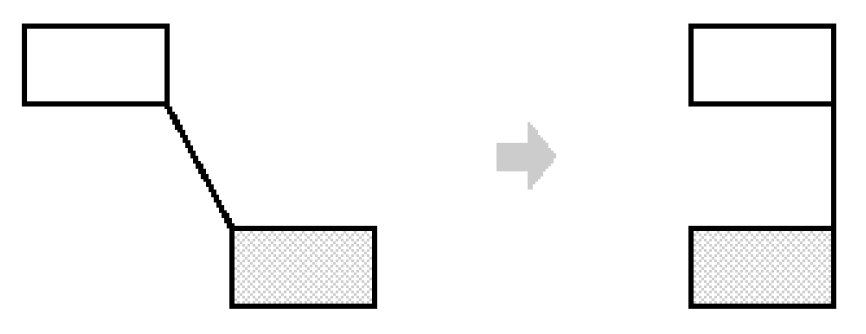
\includegraphics[scale=0.4]{motivation2.png}
\end{center}
\end{frame}
%-------------------------------------------------------------------------------------------------

%-------------------------------------------------------------------------------------------------
\begin{frame}\frametitle{Մոտիվացիան}
\begin{center}
    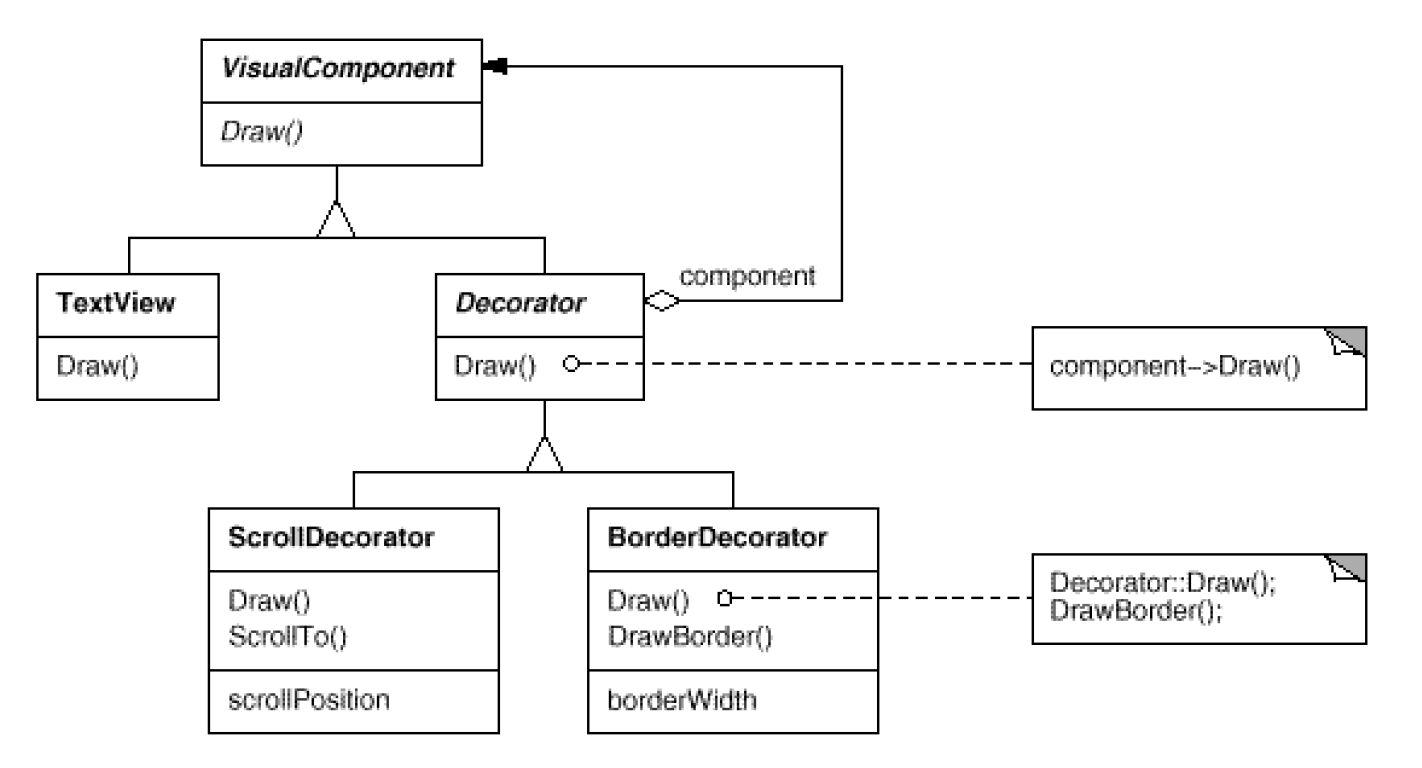
\includegraphics[scale=0.4]{motivation3.png}
\end{center}
\end{frame}
%-------------------------------------------------------------------------------------------------

%-------------------------------------------------------------------------------------------------
\begin{frame}\frametitle{Մոտիվացիան}
\begin{center}
    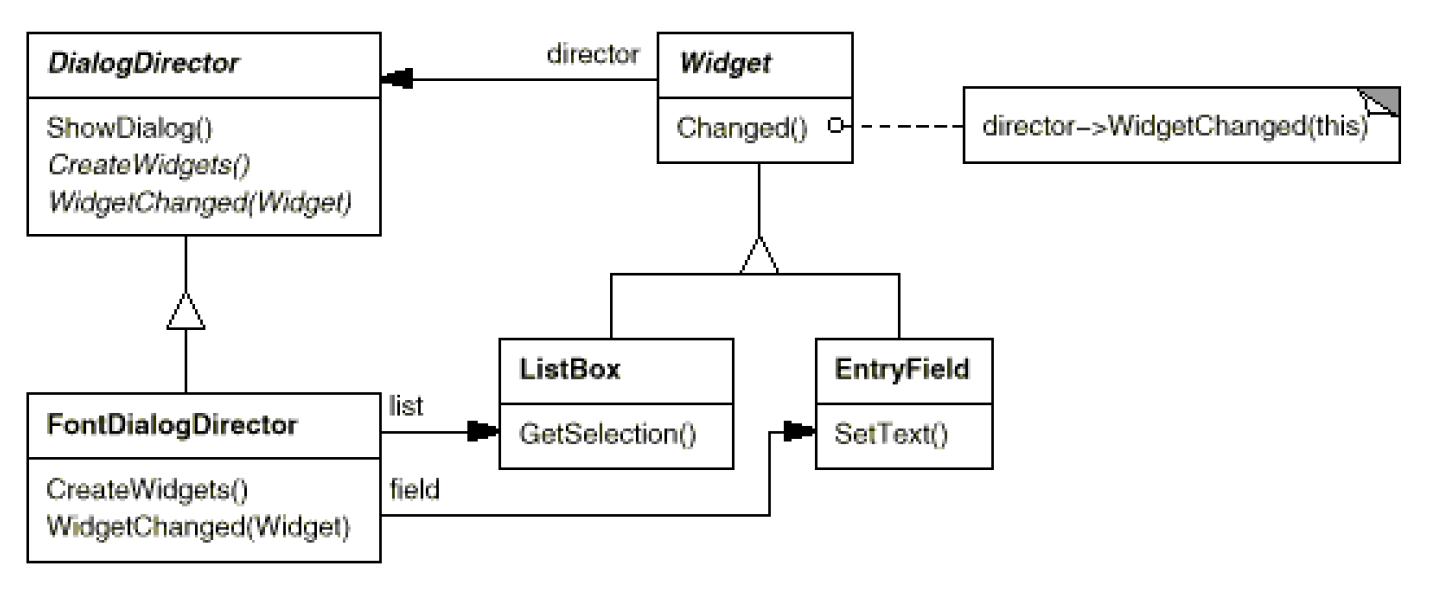
\includegraphics[scale=0.4]{motivation4.png}
\end{center}
\end{frame}
%-------------------------------------------------------------------------------------------------

\subsection{Կիրառելիությունը}
%-------------------------------------------------------------------------------------------------
\begin{frame}\frametitle{Կիրառելիությունը}
Այս Ն.Ձ. պետք է օգտագործել երբ.
\vfill
\begin{enumerate}
    \item Մի խումբ օբյեկտներ փոխազդում են լավ սահմանված և կոմպլեքս ձևով: \vfill
    \item Օբյեկտի վերօգտագործումը դժվար է նրա\\ շատ օբյեկտների հետ
    փոխազդեցության հետևանքով: \vfill
    \item Շատ օբյեկտների մեջ բաժանված վարվելակերպը պետք է փոփոխելի լինի
    առանց մեծ քանակով ենթադասեր ստեղծելու:
\end{enumerate}
\end{frame}
%-------------------------------------------------------------------------------------------------

\section{Կառուցվածքը}
%-------------------------------------------------------------------------------------------------
\begin{frame}\frametitle{Կառուցվածքը}
\begin{center}
    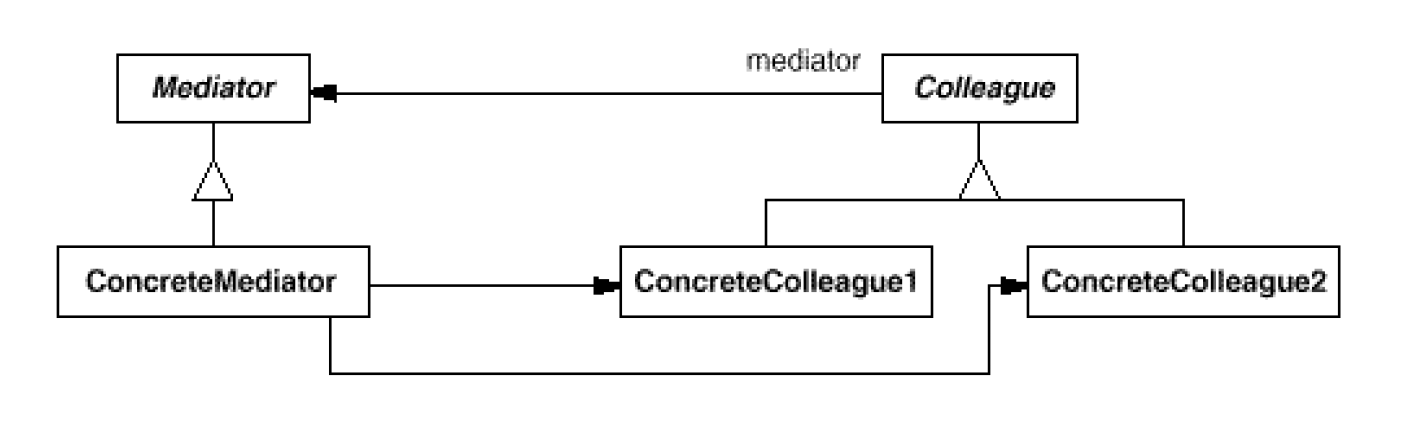
\includegraphics[scale=0.4]{structure1.png}
\end{center}
\end{frame}
%-------------------------------------------------------------------------------------------------
%-------------------------------------------------------------------------------------------------
\begin{frame}\frametitle{Կառուցվածքը}
\begin{center}
    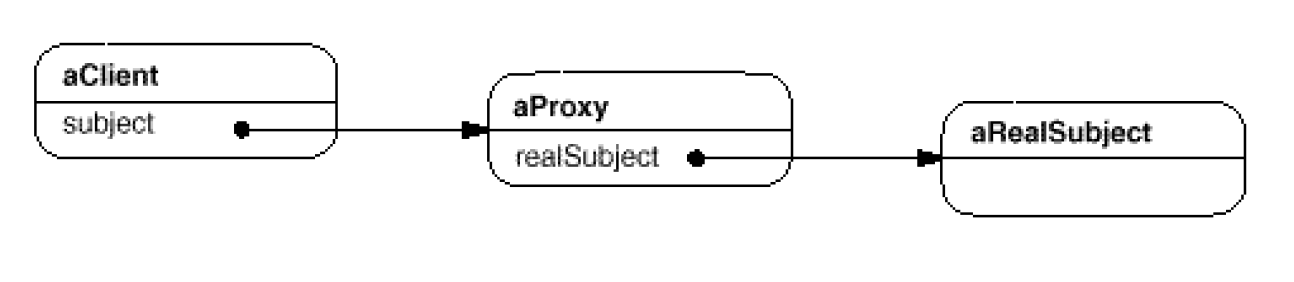
\includegraphics[scale=0.4]{structure2.png}
\end{center}
\end{frame}
%-------------------------------------------------------------------------------------------------

\subsection{Հետևանքները}
%-------------------------------------------------------------------------------------------------
\begin{frame}\frametitle{Հետևանքները}
Այս Ն.Ձ. ունի հետևյալ առավելություններն ու թերությունները.
\vfill
\begin{enumerate}
    \item Նվազեցնում է ժառանգության անհրաժեշտությունը: \vfill
    \item Բաժանում է գործընկեր դասերին: \vfill
    \item Պարզեցնում է օբյեկտների հաղորդակցումը: \vfill
    \item Աբստրակտացնում է օբյեկտների փոխհամագործակցությունը: \vfill
    \item Կենտրոնացնում է ղեկավարումը:
\end{enumerate}
\end{frame}
%-------------------------------------------------------------------------------------------------

\section{Իրականացումը}
%-------------------------------------------------------------------------------------------------
\begin{frame}\frametitle{Իրականացումը}
\begin{enumerate}
    \item Աբստրակտ Mediator դասի բացակայություն: \vfill
    \item Collegue-Mediator հաղորդակցություն:
\end{enumerate}
\end{frame}
%-------------------------------------------------------------------------------------------------

\subsection{Օրինակ}
%-------------------------------------------------------------------------------------------------
\begin{frame}[fragile]\frametitle{Օրինակ}
\begin{english}
\begin{minted}{cpp}
class DialogDirector {

public:
    virtual ~DialogDirector();
    virtual void ShowDialog();
    virtual void WidgetChanged(Widget*) = 0;

protected:
    DialogDirector();
    virtual void CreateWidgets() = 0;
};
\end{minted}
\end{english}
\end{frame}
%-------------------------------------------------------------------------------------------------

%-------------------------------------------------------------------------------------------------
\begin{frame}[fragile]\frametitle{Օրինակ}
\begin{english}
\begin{minted}{cpp}
class Widget {

public:
    Widget(DialogDirector*);
    virtual void Changed();
    virtual void HandleMouse(MouseEvent& event);

private:
    DialogDirector* director;
};

void Widget::Changed () {
    director->WidgetChanged(this);
}
\end{minted}
\end{english}
\end{frame}
%-------------------------------------------------------------------------------------------------

%-------------------------------------------------------------------------------------------------
\begin{frame}[fragile]\frametitle{Օրինակ}
\begin{english}
\begin{minted}{cpp}
class ListBox : public Widget {

public:
    ListBox(DialogDirector*);

    virtual const char* GetSelection();
    virtual void SetList(List<char*>* listItems);
    virtual void HandleMouse(MouseEvent& event);

    // Other methods
};
\end{minted}
\end{english}
\end{frame}
%-------------------------------------------------------------------------------------------------

%-------------------------------------------------------------------------------------------------
\begin{frame}[fragile]\frametitle{Օրինակ}
\begin{english}
\begin{minted}{cpp}
class EntryField : public Widget {

public:
    EntryField(DialogDirector*);

    virtual void SetText(const char* text);
    virtual const char* GetText();
    virtual void HandleMouse(MouseEvent& event);

    // Other methods
};
\end{minted}
\end{english}
\end{frame}
%-------------------------------------------------------------------------------------------------

%-------------------------------------------------------------------------------------------------
\begin{frame}[fragile]\frametitle{Օրինակ}
\begin{english}
\begin{minted}{cpp}
class Button : public Widget {

public:
    Button(DialogDirector*);

    virtual void SetText(const char* text);
    virtual void HandleMouse(MouseEvent& event);

    // Other methods
};

void Button::HandleMouse(MouseEvent& event) {
    // Local event handling
    Changed();
}
\end{minted}
\end{english}
\end{frame}
%-------------------------------------------------------------------------------------------------

%-------------------------------------------------------------------------------------------------
\begin{frame}[fragile]\frametitle{Օրինակ}
\begin{english}
\begin{minted}{cpp}
class FontDialogDirector : public DialogDirector {

public:
    FontDialogDirector();
    virtual ~FontDialogDirector();
    virtual void WidgetChanged(Widget*);

protected:
    virtual void CreateWidgets();

private:
    Button*     ok;
    Button*     cancel;
    ListBox*    fontList;
    EntryField* fontName;
};
\end{minted}
\end{english}
\end{frame}
%-------------------------------------------------------------------------------------------------

%-------------------------------------------------------------------------------------------------
\begin{frame}[fragile]\frametitle{Օրինակ}
\begin{english}
\begin{minted}{cpp}
void FontDialogDirector::CreateWidgets () {

    ok = new Button(this);
    cancel = new Button(this);
    fontList = new ListBox(this);
    fontName = new EntryField(this);

    // Fill the listBox with the available font names

    // Assemble the widgets in the dialog
}
\end{minted}
\end{english}
\end{frame}
%-------------------------------------------------------------------------------------------------

%-------------------------------------------------------------------------------------------------
\begin{frame}[fragile]\frametitle{Օրինակ}
\begin{english}
\begin{minted}{cpp}
void FontDialogDirector::WidgetChanged(Widget* theChangedWidget) {

    if (theChangedWidget == fontList) {

        fontName->SetText(fontList->GetSelection());

    } else if (theChangedWidget == ok) {

        // apply font change and dismiss dialog

    } else if (theChangedWidget == cancel) {

        // dismiss dialog
    }
}
\end{minted}
\end{english}
\end{frame}
%-------------------------------------------------------------------------------------------------

\section{Առնչվող Ձևանմուշները}
%-------------------------------------------------------------------------------------------------
\begin{frame}\frametitle{Առնչվող Նախագծման Ձևանմուշները}
\begin{itemize}
    \item Facade \vfill
    \item Observer
\end{itemize}
\end{frame}
%-------------------------------------------------------------------------------------------------

\end{document}
